

\iffalse
% Extra FD notes
    \subsubsection{Forward Detector}
        Overview:
        \subsubsection{HTCC}
            Used basically as an electron trigger. Composed of 60 lightweight ellipsoidal mirrors, that focus Cherenkov light onto eigh 5-inch phototubes (48 channels on entire HTCC). Working gas is CO2 at STP (n=1.0005, $\theta_{max}$ = 1.7 degrees, covers 5 to 35 degrees, 2$\pi$ in azimuth. Active area 2.4 meters in diameter. Electron signal threshold is 15 MeV, charged pion threshold is 5 GeV. 99.9\% electron detection efficiency vs. pions. 15 feet in diameter, 6 feet long. Mirror thickness is 0.1 g/$cm^2$. Kaons have no signal, as they would need 16 GeV to generate a signal. Uses Winston cones to increase collection efficiency. 20 photoelectrons per electron in HTCC, 25\% quantum efficency. The PMTs have 14 dynodes, gain of about $10^7$. HTCC material budget 0.135 g/$cm^2$
            
            									
			 \begin{figure}[H]
    			\centering
    			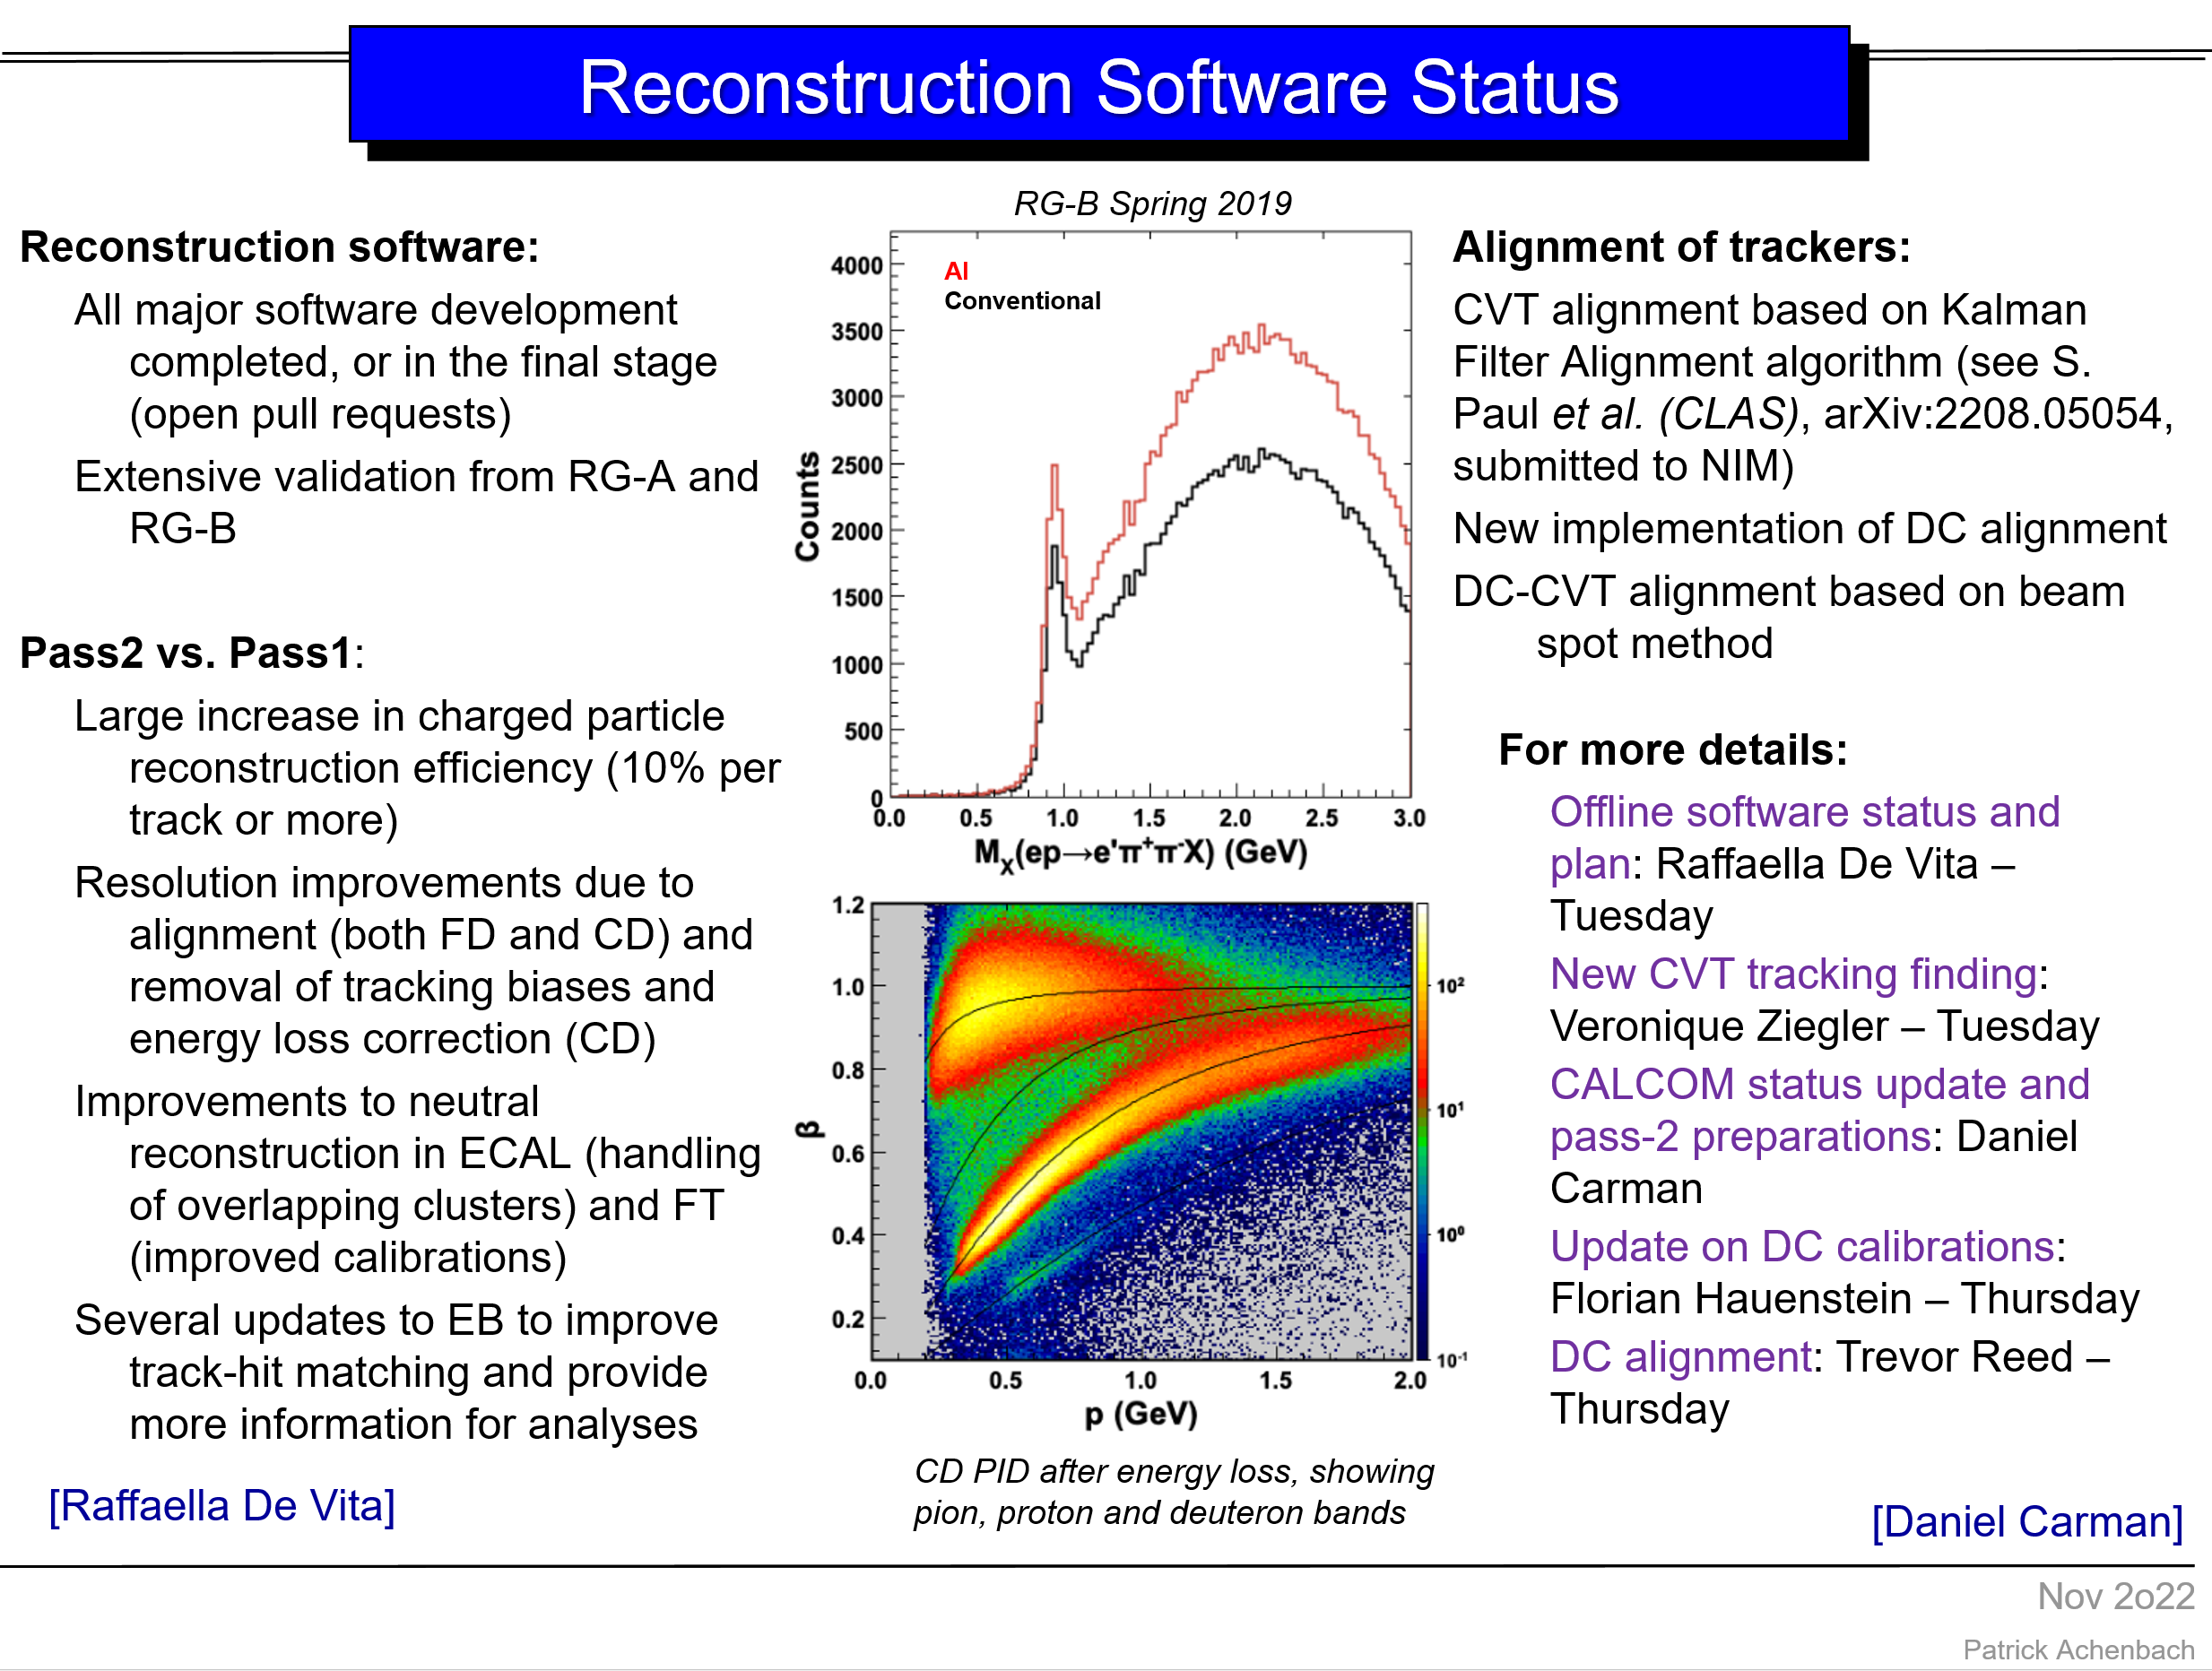
\includegraphics[width=12cm]{Chapters/Ch2-Experiment/recon_pid/pass2vpass1.png}
    			%%%\caption{SVT Strip}
			\end{figure}
			
						
									

			
			

        
        \subsubsection{Torus}
        Outbending allows for lower Q2 measurements, inbending allows for slighly higher Q2 measurements. 

            6 coil torus, 4k amps, 3.5 Tesla torodial field, supercritical LHe cooled. 14.2 Megajoules stored energy. 2 Henries of inductance. Field strongest at small angles, weakest at large angles. 
              Inbending vs out bending:
        I have been wondering about this as well. All I know is that inbending and outbending have different acceptances.
        So, I guess some channels prefers inbending while the others do outbending? I’m not sure though. FX claims outbending results have better quality for these days. 
            									
			 \begin{figure}[H]
    			\centering
    			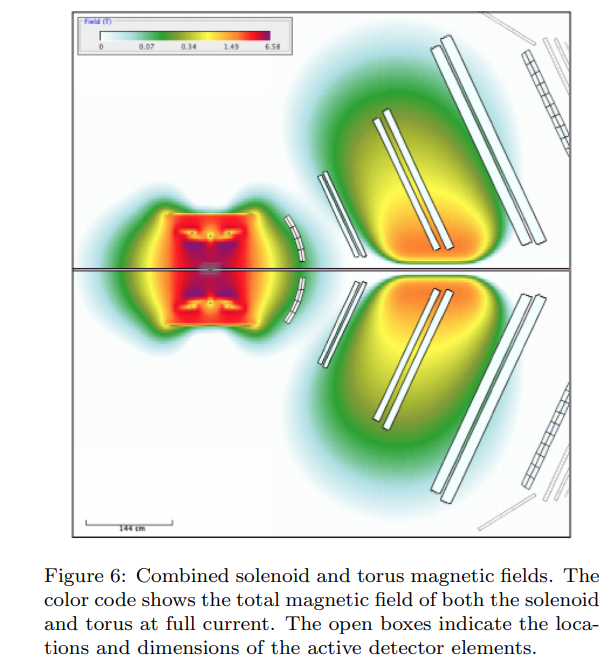
\includegraphics[width=12cm]{Chapters/Ch2-Experiment/clas-12-exp/clas-detectors/fd/pics/torus.png}
    			%%%\caption{SVT Strip}
			\end{figure}
                        

        
        \subsubsection{Drift Chambers}
            There are 3 layers of drift chambers, each with 6 sections. Each chamber has 2 superlayers of 6 layers by 112 wires, for a total of 24,192 wires. (Structure is 112 wires * 6 layers * 2 superlayers * 18 DC sections = 24,192 wires). Physical wire sectioning looks like:\\
            (IIIIII)-(IIIIII)---(IIIIII)-(IIIIII)---(IIIIII)-(IIIIII) x 6 sectors\\
            Where each "I" is a layer of 112 wires.\\
            Spatial resolution is 300 $\mu$ m, angular coverage 5-40 degrees. Momentum resolution $\Delta$p/p < 1\%, angular resolution is 1 mrad in theta, 1mrad/$\sin{\theta}$ for phi. The Drift Chambers are located 2, 3, and 4 meters from the gas mixture is 90/10 Argon/CO2. Time resolution = ?\\
            DC specifics: 30 micron diameter tungsten sense wires, 80 micron Cu-Be field wires, 140 micron Cu-Be guard wires. 20 g tension on sense, 62 g tension of field, 180 g on guard. Max sag calculated to be on order of 10 microns.
            
            									
			 \begin{figure}[H]
    			\centering
    			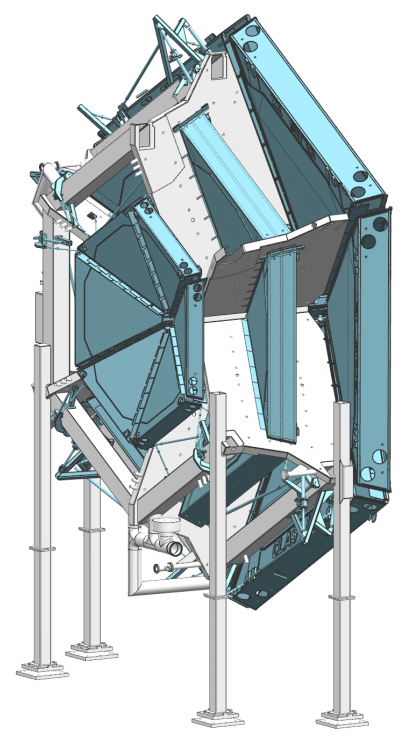
\includegraphics[width=12cm]{Chapters/Ch2-Experiment/clas-12-exp/clas-detectors/fd/pics/drift-chambers.png}
    			%%%\caption{SVT Strip}
			\end{figure}    

            
        \subsubsection{LTCC}
            6 sectors, perfluorobutane ($C_4F_10$) $\longrightarrow$ n = 1.0013 $\longrightarrow$ $\theta_{max}$ = 3 degrees. Electron threshold 9 MeV, pion threshold 2.7 GeV, Kaon threshold 9.4 GeV. Allows for good pion/kaon discrimination from 3.5 Gev to 9 GeV. \\
            Each section has 108 mirrors, 36 winston cones, and 36 PMTs. Mirror is aluminium with $MgF_2$ coating. Kevlar support structure. Perflourobutane is 100\% transparent above 220 nm light. 
            
            
						
									
			 \begin{figure}[H]
    			\centering
    			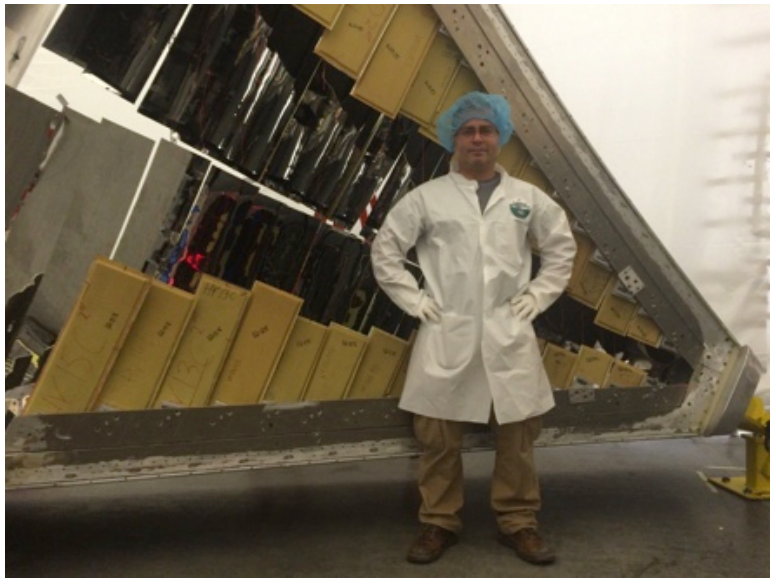
\includegraphics[width=12cm]{Chapters/Ch2-Experiment/clas-12-exp/clas-detectors/fd/pics/ltcc.png}
    			\caption{Low Threshold Chrenkov Counter}
			\end{figure}
			
			

			
        \subsubsection{RICH}
            Provides PID in the range of 3-8 GeV, replacing one sector of LTCC (right middle sector). Pion/Kaon rejection factor > 500, Kaon/Proton rejection factor > 100. Covers 5 to 25 degrees in theta, uses aerogel (n=1.05 $\longrightarrow$ $\theta_{max}$ = 18 degrees). Pion threshold 460 MeV, Kaon threshold 1.6 GeV. Read out by 64 channel photomultipliers. $\beta_{min}$=0.95, $\gamma_{min}$ = 3.3
            
            What is angular resolution?
            
            Reminder of relevant equation:
            \begin{equation}
                \cos{\theta} = \frac{1}{\beta n} \longrightarrow \theta = \arccos{\frac{1}{\beta n}}
            \end{equation}
            
            \begin{equation}
                \gamma = \frac{1}{\sqrt{1-\beta^2}} \longrightarrow \beta = 1-\frac{1}{1-\gamma^2} 
            \end{equation}
            
            \begin{table}[H]
                \centering
                    \begin{tabular}{llll}
                         & momentum & $\sim \gamma$ & $\theta$  \\
                    pion & 3        & 21            & 17.4                      \\
                    kaon & 3        & 6             & 12                        \\
                         &          &               &                         \\
                    pion & 5      & 36            & 17.6                      \\
                    kaon & 5       & 10.1             & 15.9                        \\
                         &          &               &                          \\
                    pion & 8      & 57.1            & 17.7                      \\
                    kaon & 8       & 16             & 17.1                        \\
                    
                    \end{tabular}
            \end{table}
            
        
            
            
            
            \begin{table}[H]
                \centering
                    \begin{tabular}{lll}
                        Detector    &   Scintillator                         &   PMT   \\
                        FTOF - 1a   &     \textcolor{blue}{BC-408}           &   \textcolor{red}{Phillips XP2262, EMI 9954A}\\
                        FTOF - 1b   &     \textcolor{red}{BC-404}           &   \textcolor{blue}{Hama. R9779} \\
                        FTOF - 2    &     \textcolor{blue}{BC-408}           &   \textcolor{magenta}{EMI 4312KB} \\
                        PCAL        &     FNAL                               &   \textcolor{red}{Hama. R6095}\\
                        ECAL        &     \textcolor{cyan}{BC-412}           &   \textcolor{red}{Philips XP2262, EMI 9954}\\
                        CND         &     \textcolor{red}{EJ-200}            &   \textcolor{cyan}{Hama. R10533} \\
                        CTOF        &     \textcolor{blue}{BC-408}           &   \textcolor{green}{Hama. R2083} \\
                        HTCC        &         N/A                            &   ET 9823QKB \\
                        LTCC        &           N/A                          &   200 Photonis XP 4500B\\
                        LTCC        &              N/A                       &   16 Photonis XP 4508 (Quartz Window)\\
                    \end{tabular}
            \end{table}
            
            *ET stands for Electron Tube, a company. Could not find a spec sheet for this PMT type. 
            ** Could not find spec sheets for either HTCC, or LTCC PMTs. 
       
               
            \begin{table}[H]
                \centering
                    \begin{tabular}{lllllll}
                        Scintillator                    & Detectors             &   Principal Use/Features      &   L.O. & WME & R/D Time & L.A. Length \\
                         \textcolor{red}{BC-404}       &  FTOF-1b              &   Fast Counting                   &           68    &   408    & 0.7/1.8           &   140   \\
                         \textcolor{blue}{BC-408}       &  FTOF-1b,2,CTOF       &   TOF - Large Area                &           64    &   425   &   0.9/2.1         &   210  \\
                        \textcolor{cyan}{BC-412}        &  ECAL                 &   Large Area                      &           60   &   434 &   1.0/3/3         &   210\\
                        \textcolor{red}{EJ-200}        &  CND                  &   Long attenuation, fast   &           64     &   425       &   0.9/2.1         &   380   \\
                    \end{tabular}
            \end{table}   
            
            L.O - Light Output - \% Anthracene
            WME - Wavelength Maximum of Emitted Photons
            R/D Time - Rise / Decay time (ns)
            L.A. Length - light attenuation length (cm)
             
             All scintillators have a PVT (Polyvinyltoluene) base. 
             
             EJ-200:          200 -- 10K photons per 1 MeV. 
             
             Thermal effects: EJ-200 loses 5\% of its light output between 20 degrees C and 60 degrees C. No change between -60 to 20 degrees C. 
            
            \begin{table}[H]
                \centering
                %\begin{localsize}{10}
                \scalebox{0.9}{
                    \begin{tabular}{llllllll}
                        PMT                                         & Det.                      &       TS/A    &   WVE         &   PHTC    &   DNY     &       Anode  &    Time Resp.\\ 
                        \textcolor{red}{Hama. R6095}               &  PCAL                     &       28/25   &   300/420/650 & BA/BSG & B\&L/11/2.1  &   1500/0.1    & 4/30/3    \\
                        \textcolor{blue}{Hama. R9779}               &  FTOF-1b                  &       51/46   &   300/420/650 & BA/BSG & LF/8/0.5     &   1750 /0.1   & 1.8/20/0.25 \\
                        \textcolor{cyan}{Hama. R10533}              &  CND                      &       51/46   &   300/420/650 & BA/BSG & LF/10/4.2    &   1000/0.1    &  2/24    \\   
                        \textcolor{green}{Hama. R2083}              &  CTOF                     &       51/46   &   300/420/650 & BA BSG & LF/8/2.5     &   3000/0.2    & 0.7/16/    \\
                        \textcolor{red}{Phillips XP2262}            &  FT1a ECAL            &    &&&&&\\
                        \textcolor{red}{EMI 9954A}                  &  FT1a ECAL            &    &&&&&\\
                        \textcolor{magenta}{EMI 4312KB}             &  FTOF-2                   &    &&&&&\\
                    \end{tabular}}
                %\end{localsize}
            \end{table} 
            
            No spec sheets could be found for the PMTs used in the TFOT1a, ECAL, or FTOF-2.
            Typical dark currents for all PMTs are 100 nA. 
        
            
            Tube size / photocathode area (diameter in mm)
            Wavelength short / peak / long (nm)
            Photocathode / window material (BA = Bialkali, BSG = Borosilicate Glass)
            Dynode structure / stages / gain  LF = Linear-focused, B\&L = Box and line / / Gain - Gain x 10$^6$
            Anode to Cathode Voltage / Anode Current  - Volts / mA
            Rise / transit time/time spread in ns
            
            
            
            \href{https://www.hamamatsu.com/eu/en/product/type/R10533/index.html}{R10533 PMT}
            \href{https://www.hamamatsu.com/eu/en/product/type/R2083/index.html}{R2083 PMT}
            \href{https://pdf1.alldatasheet.com/datasheet-pdf/view/212324/HAMAMATSU/R9779.html}{R9779 PMT}
            \href{https://www.sphere.bc.ca/test/phototubes2/ham/r6095.pdf}{R6095 PMT}
            
            
            
            
            
            
            
            
            
            \href{https://eljentechnology.com/products/plastic-scintillators/ej-200-ej-204-ej-208-ej-212}{CND Scintillator}
            
            
            \href{https://www.crystals.saint-gobain.com/sites/imdf.crystals.com/files/documents/bc400-404-408-412-416-data-sheet.pdf}{BC Scint Specs from Saint Gobain}
            
            
            \href{https://www.hamamatsu.com/eu/en/product/type/R10533/index.html}{CND PMT}
            
            
            \href{https://www.hamamatsu.com/us/en/product/type/R2083/index.html}{CTOF PMT Spec sheet}
            Bialkali photocathode, 8 dynodes, 2.5*10$^6$ typical gain
            Linear-focused dynode structure
            Window material Borosilicate glass
            peak wavelength 420 nm, range from 300 to 650 nm. Max anode to cathode voltage of 3500 V, made anode current of 0.2 mA. Dark current around 100 nA. 
            
            
        
        \subsubsection{FTOF}
            Used for PID, three layer system - 1a, 1b, and 2. Has a design resolution of 60 ps to 160 ps. Average scintillation rate 250 kHz. Pion/Kaon separation up to 2.8 GeV, Kaon Proton separation up to 4.8 GeV, pion proton separation up to 5.4 GeV. \\
            6 meters away from target.
            Time resolution of 80 ps less than 36 degrees, 150 ps greater than 36 degrees. PMTs are shileded from CLAS12 torus. 6 sectors, plastic scintillator, double sided PMT readout. 3 panesl - 1a - 23 counters, 1b - 62 counters, 2 - 5 counters. \\
            15cm wide x 5 cm deep x 33 cm up to 376 cm long.\\
            20-30 cm up to 15x5 130 ps\\
            350-400 cm 6x6 60 ps\\
            370 to 430 cm, 22x5cm, 150 ps\\
            
            									

		
			 \begin{figure}[H]
    			\centering
    			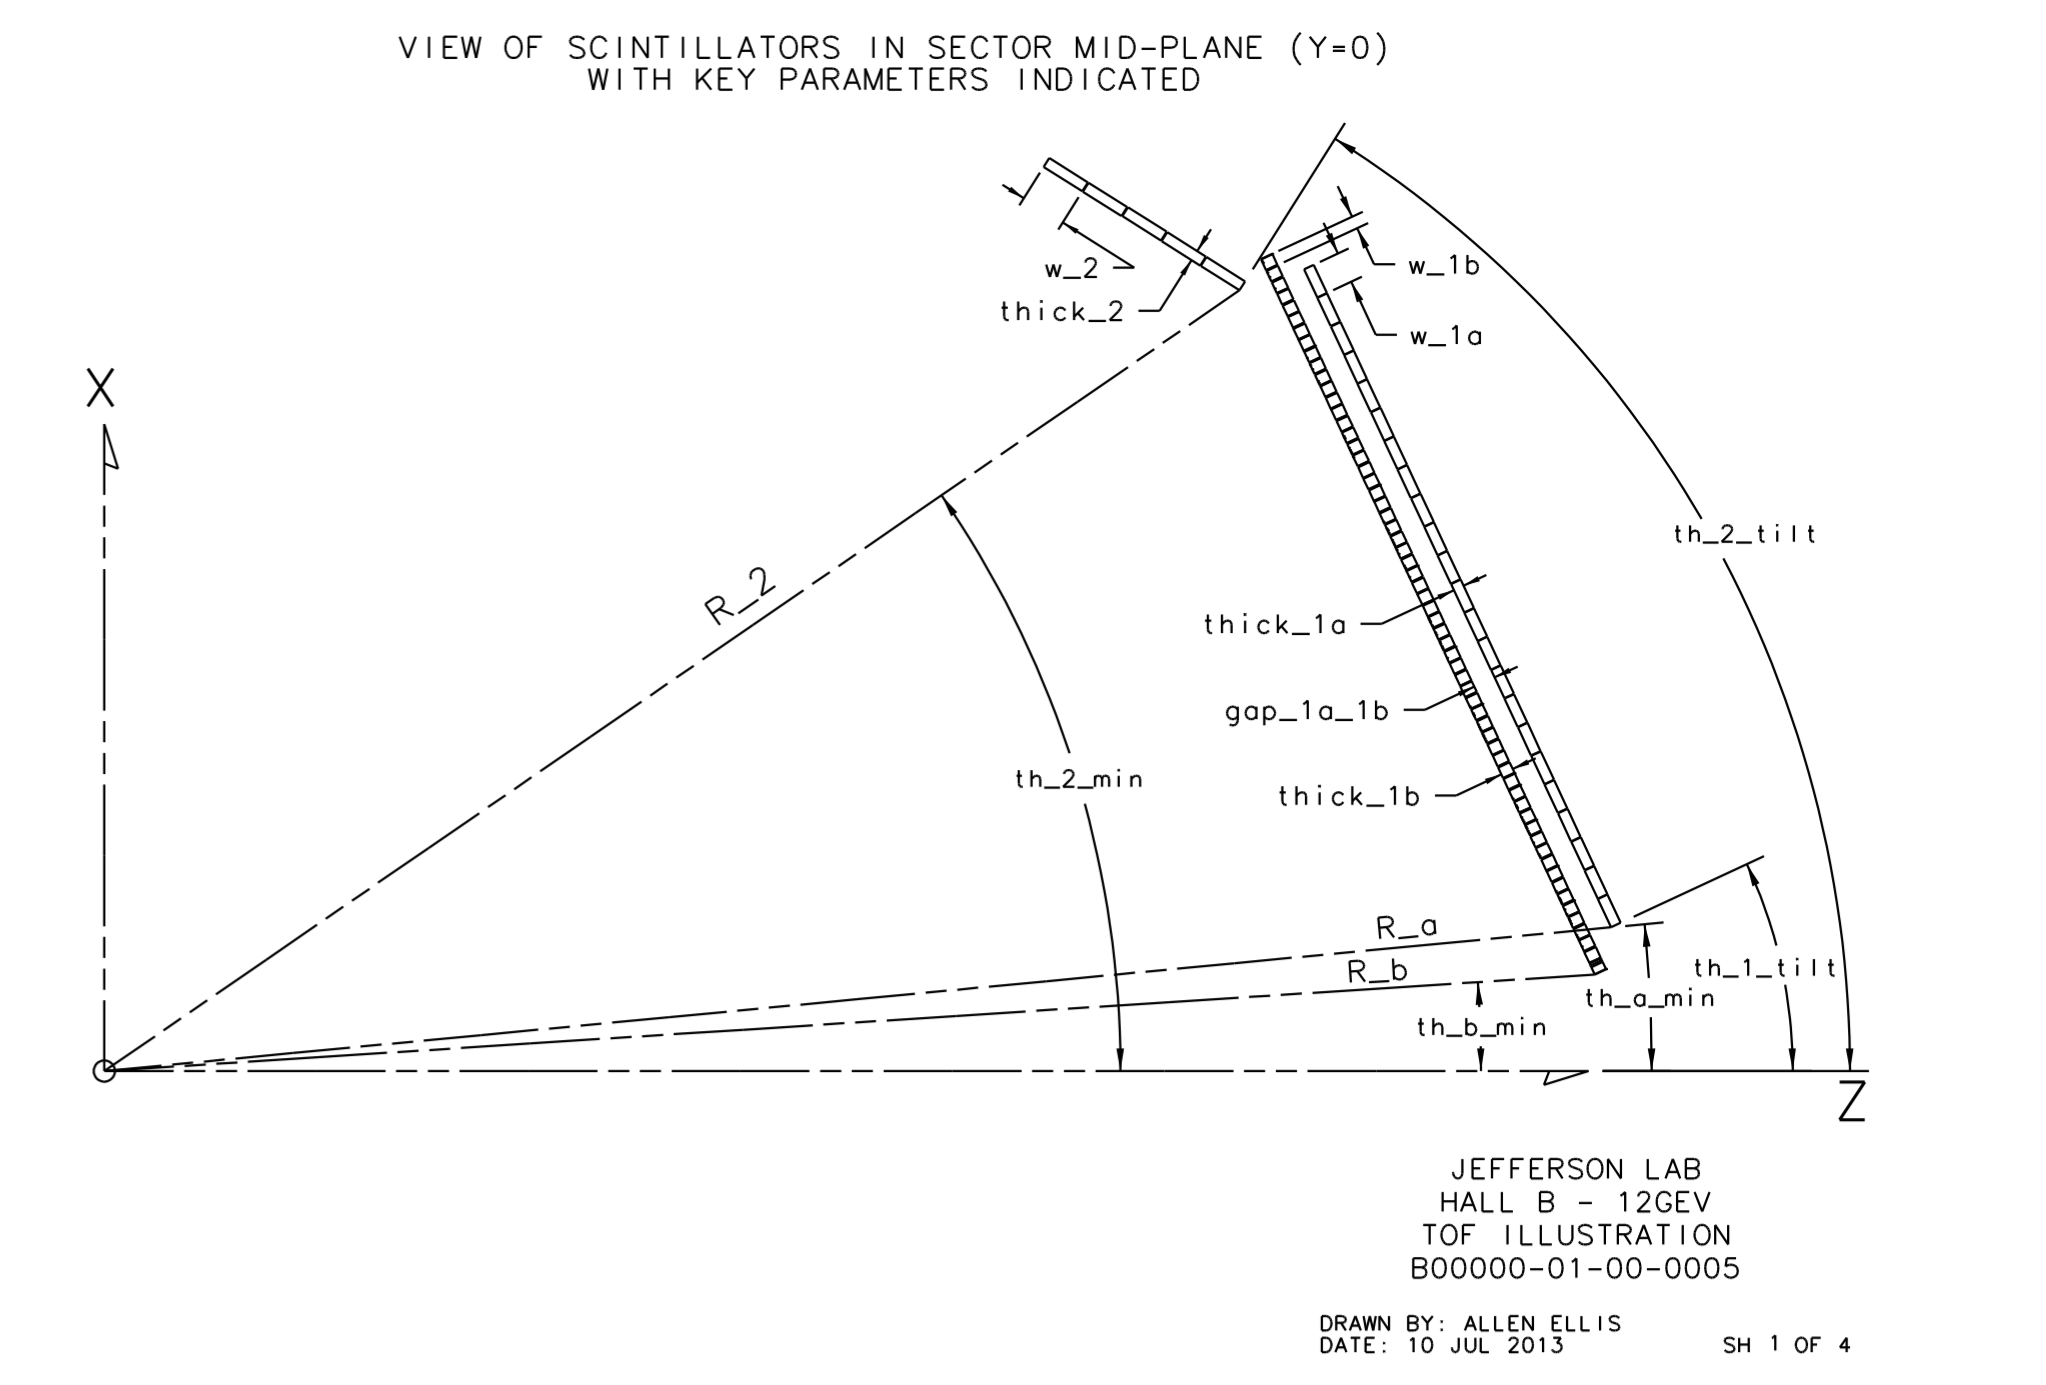
\includegraphics[width=12cm]{Chapters/Ch2-Experiment/clas-12-exp/clas-detectors/fd/pics/clas12-ftof-geom.png}
    			%%%\caption{SVT Strip}
			\end{figure}
			
			
            
            The timing resolution minimums are for being close to the beam axis where particles are moving faster, and farther out from the beamline (larger theta) particles are moving slower so a less resolved time difference is acceptable. 
            
            \paragraph{1a}
                Coverage is 50\% at 5 degrees to 85\% at 35 degrees\\
                Dimensions: L 32.3 cm to 376.1 cm, wxh = 15x5 cm\\
                Material BC-408\\
                PMTS: EMI 9954A, Phillips XP2262\\
                Time resolution 90 - 160 ps small bar to big bars\\
            \paragraph{1b}
                Coverage is 50\% at 5 degrees to 85\% at 35 degrees\\
                Dimensions: L 17.3 cm to 407.9 cm, wxh = 6x6 cm\\
                Material BC-404 (first half) and BC-408\\
                PMTS: Hamamatsu R9779\\
                Time resolution 60-110 ps small bar to big bars\\
            \paragraph{2}
                Coverage is 85\% at 35 degrees to 90\% at 45 degrees\\
                Dimensions: L 371.3 cm to 426.2 cm, wxh = 22x5 cm\\
                Material BC-408\\
                PMTS: EEMI 4312KB\\
                Time resolution 140 - 165 ps small bar to big bars\\
           
           
            For more FTOF specifcications, look \href{https://www.jlab.org/Hall-B/ftof/notes/ftof_geom.pdf}{here} 
                
            FTOF two panels:
Official answer from CLAS12 FTOF NIM paper:
"For tracks that pass through both arrays the combined time information (described in Ref. [10]) is used and results in a 20% improvement compared to using the hit information from panel-1b alone.”, https://www.sciencedirect.com/science/article/pii/S0168900220302102

I guess this is the right answer though:
1a is recycled one from CLAS while 1b is new one.
            
            
        \subsubsection{PCal and ECal}
            ECal from CLAs could only contain showers with E < 5 GeV. Above 5.5 GeV, couldn't resolve neutral pion gamma gamma angle, so needed PCAL. PCAL is 7 meters from target, ECAL is 7.5 M from target. EC segmentation 10 cm, PCAL finer segmentation. PCal 5.5 radiation lengths. 20.5 radiation lengths total. Both are sampling calorimeters, with PB and scintillator layers. The CLAS ECAL was resused and a new PCAL was installed in front of it. Primarily used for identification of electrons, photons, gamma gamma decays from pions, and neutrons. They are sampling calorimeters with six moduels. Each module has a triangular shape with 54 (15/15/24 - PCAL/ECALinner/ECALouter) layers of 1 cm htick scintillators segmented into 4.5/10 cm (PCAL/ECAL) wide strips and sandwiched between 2.2 mm thick lead sheets. The total thickness is about 20.5 radiation lengths. \\
            \indent Scintillator layers are grouped into three readout views with 5/5/8 PCAL/ECinner/ECouter, layers per view providing several cm resolution of energy clusters. Light from each scintillator readout group is routed to PMTs via flexible optical fibers.\\
            Overall perfomance:\\
            Energy resolution of 10\%, position resolution of 2 cm, time resolution of 500 ps. \\
            Are these the real statistics? Because they seem like BS.
            
            
            
            \begin{figure}[H]
    			\centering
    			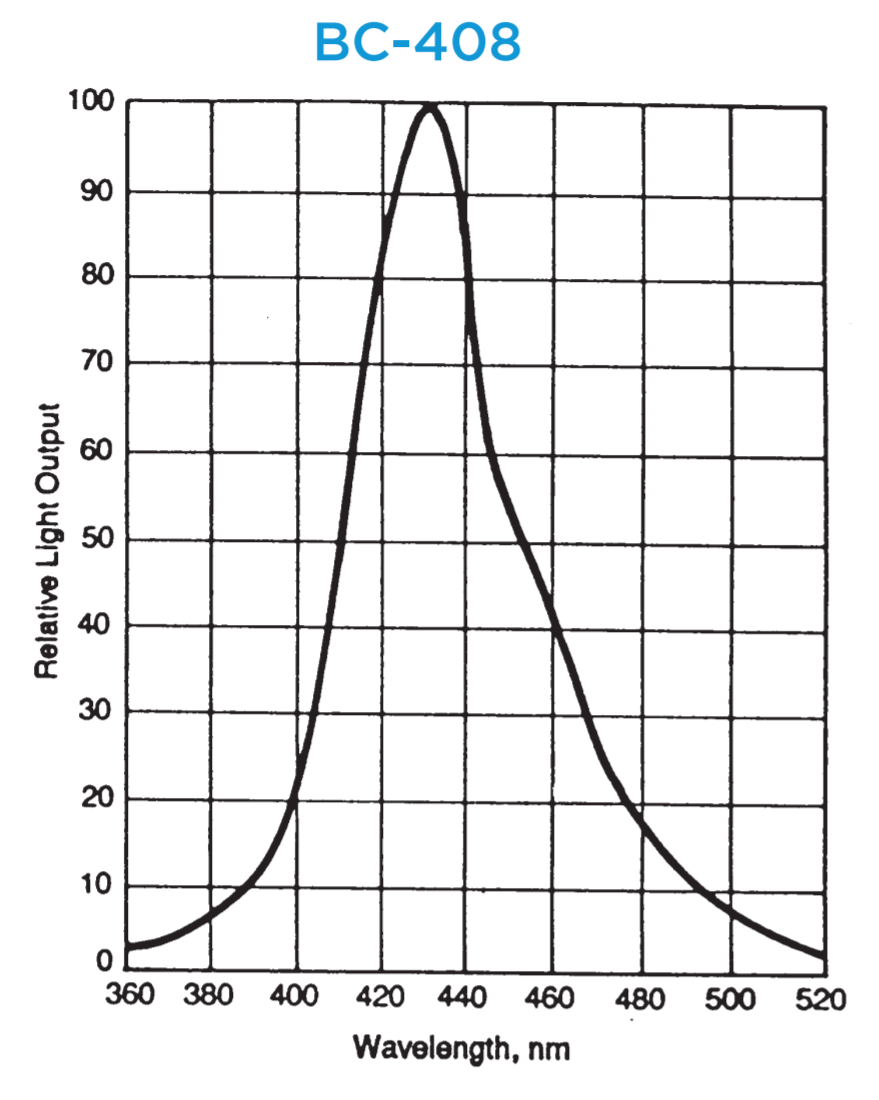
\includegraphics[width=12cm]{Chapters/Ch2-Experiment/clas-12-exp/clas-detectors/fd/pics/sample-BC-408-emission-spectra.png}
    			%\caption{BC 408 Emission Spectra}
			\end{figure}
			
            						


			 \begin{figure}[H]
    			\centering
    			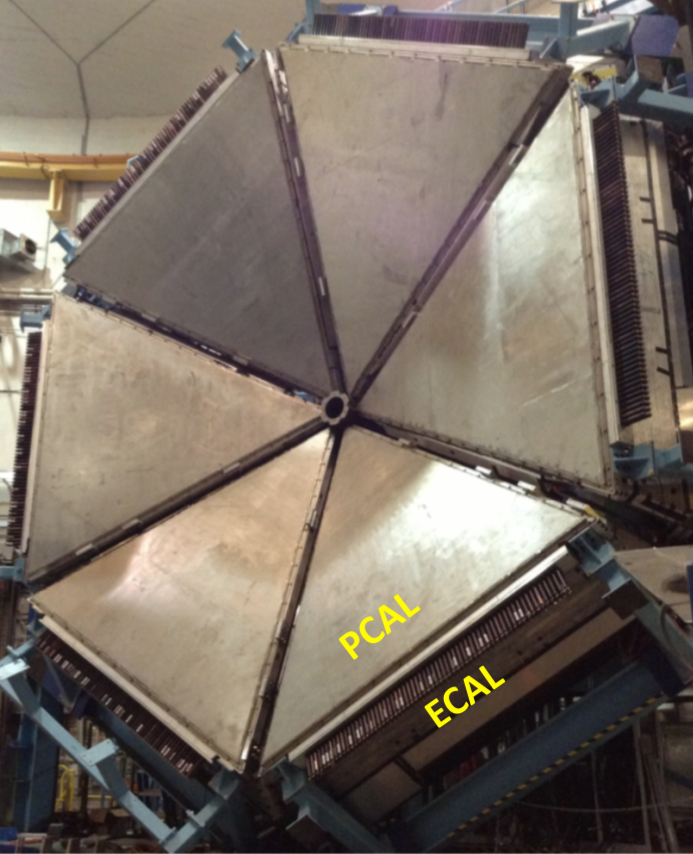
\includegraphics[width=12cm]{Chapters/Ch2-Experiment/clas-12-exp/clas-detectors/fd/pics/clas12-pcal-ecal.png}
    			%%%\caption{SVT Strip}
			\end{figure}
			
			
        \subsubsection{PCAL}
                \indent 50\% coverage at 5 degrees, 85\% coverage at 35 degrees. 15 scintillators, 14 lead layers, per module. 1200 scintillator strips, 1x4.5 cm$^2$ up to 432 cm long, with two holes along the strip, and 0.25 mm TiO2 coating (reflective coating)\\
                Lead sheets are 2.2 mm thick. Readout by fibers into 1 inch PMTs, Hamamatsu R6095. Light yield is 11-12 photo-electrons per MeV. 
                
                PCAL scinitllator was manufactured at the FNAL-NICADD Extrusion Line Facility. Polystyrene base was Dow STYRON 663 W, primary dopant is 2,5 -diphenyloxazole (PPO, 1\% by weight) - this is the organic scintillator, peaks at 385 nm:
                
                
            \begin{figure}[H]
    			\centering
    			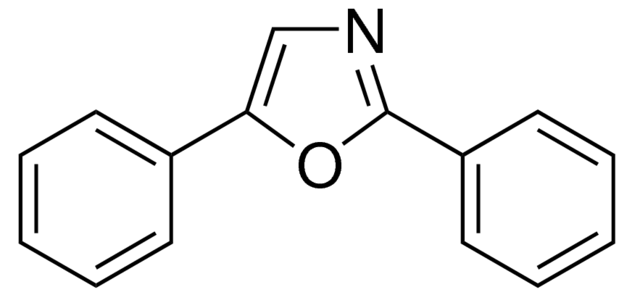
\includegraphics[width=12cm]{Chapters/Ch2-Experiment/clas-12-exp/clas-detectors/fd/pics/2-5-diphenyloxazole.png}
    			%\caption{2,5-diphenyloxazole}
			\end{figure}
                
                The Secondary dopant is 1,4 bis (5-phenyloxazol- 2-yl) benzene (POPOP, 0.03\% by weight) - also scintillator, peaks at 410 nm. 
                
                                
            \begin{figure}[H]
    			\centering
    			
\includegraphics[width=12cm]{Chapters/Ch2-Experiment/clas-12-exp/clas-detectors/fd/pics/popop.png}
    			%\caption{1,4 bis (5-phenyloxazol- 2-yl) benzene}
			\end{figure}
                
                
                
                A reflective surface coating of polystyrene with 12\% TiO2 with 0.25 mm nominal thickness was co-extruded. 
                
                Cast plastic scintillator costs about \$50 per kg, while extruded scintillator is significantly lower in price - about \$10 per kg. 
                
                \href{https://lss.fnal.gov/archive/2005/pub/fermilab-pub-05-344.pdf}{Interesting write up on FNAL Scintillator extrustion}


\href{https://www.sciencedirect.com/science/article/pii/S0168900220300309?via\%3Dihub}{PCal Technical Report}
\href{https://www.sciencedirect.com/science/article/pii/S0168900200009967}{ECal Technical Report}

                
        \subsubsection{ECAL}
                \indent 50\% coverage at 5 degrees, 85\% coverage at 35 degrees. 39/38 scintillators / lead layers per module. 216 readout channels per module, 1200 strips per module. Strips are 1x10to12cm$^2$ by up to 441 cm long, BC-412 (plastic scintillator with high light output, longest light attentuation length, \href{https://www.crystals.saint-gobain.com/products/bc-408-bc-412-bc-416}{cheap!} ). Lead sheets are 2.4 mm thick. Read out by fiber into 2 inch PMTs, Phillips XP2262 and EMI 9954. 3-4 photoelectrons/MeV deposited energy. 
\fi